\documentclass[10pt]{article}
 
\usepackage[margin=1in]{geometry} 
\usepackage{amsmath,amsthm,amssymb, graphicx, multicol, array}
\usepackage{enumitem}
\usepackage{hyperref}
 
\newcommand{\N}{\mathbb{N}}
\newcommand{\Z}{\mathbb{Z}}
 
\newenvironment{problem}[2][Problem]{\begin{trivlist}
\item[\hskip \labelsep {\bfseries #1}\hskip \labelsep {\bfseries #2.}]}{\end{trivlist}}

\date{Due: Oct 11, 2022 10pm PT}

\begin{document}
 
\title{Assignment 6}
\author{
CS 181AG: Network Algorithmics}
\maketitle

In this assignment,you will explore how to make a binary search more efficient and gain practice with packet classification by creating a small firewall. The assignment also includes a reading and writing component.

\begin{problem}{1: Improving Binary Search}
In class, we learned about how binary search can be used on prefix lengths to perform IP lookup. In this problem, we'll look at how to improve the throughput of binary search. For simplicity, we'll consider the problem of looking for elements in an array, but the results can be extrapolated to prefix lengths.

Suppose we have 7 elements total, arranged in 7 contiguous memory locations as shown below. Binary search is performed using a pointer to keep track of which element we are comparing against. While a single search takes O(log n), we wonder whether we can have multiple ongoing searches at once. However, we quickly run into a problem if multiple searches need to probe the same location in memory. 

\begin{figure}[h]
    \centering
    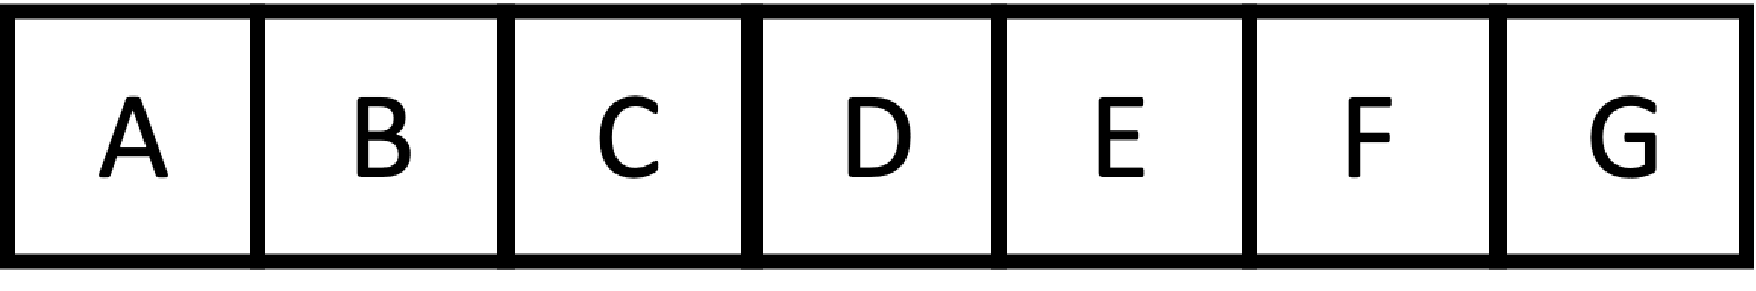
\includegraphics[scale=0.2]{figures/bin_search.pdf}
    \label{fig:bin_search}
\end{figure}

Without using extra memory, explain how we can increase the throughput of binary search lookups while avoiding the problem of multiple probes to the same memory location. What is the maximum number of searches that can be in progress simultaneously in this example?
\end{problem}

\subsection*{Answer 1:}


\begin{problem}{2: Building a Firewall}
In this problem, you will construct the rules for a small firewall and build two types of tries from your rule database.
\begin{enumerate}
    \item Let's first build the rule database for the router pictured below. It sits at the edge of a network. Two devices, P and Q, are connected to the network. S and T are two devices outside the network. The relevant IP prefixes/addresses are provided here. For simplicity, assume IPs are only 4 bits long instead of 32.
    
    Network prefix: 01*; P: 0101; Q: 0110; S: 1010; T: 1101
    
\begin{figure}[h]
    \centering
    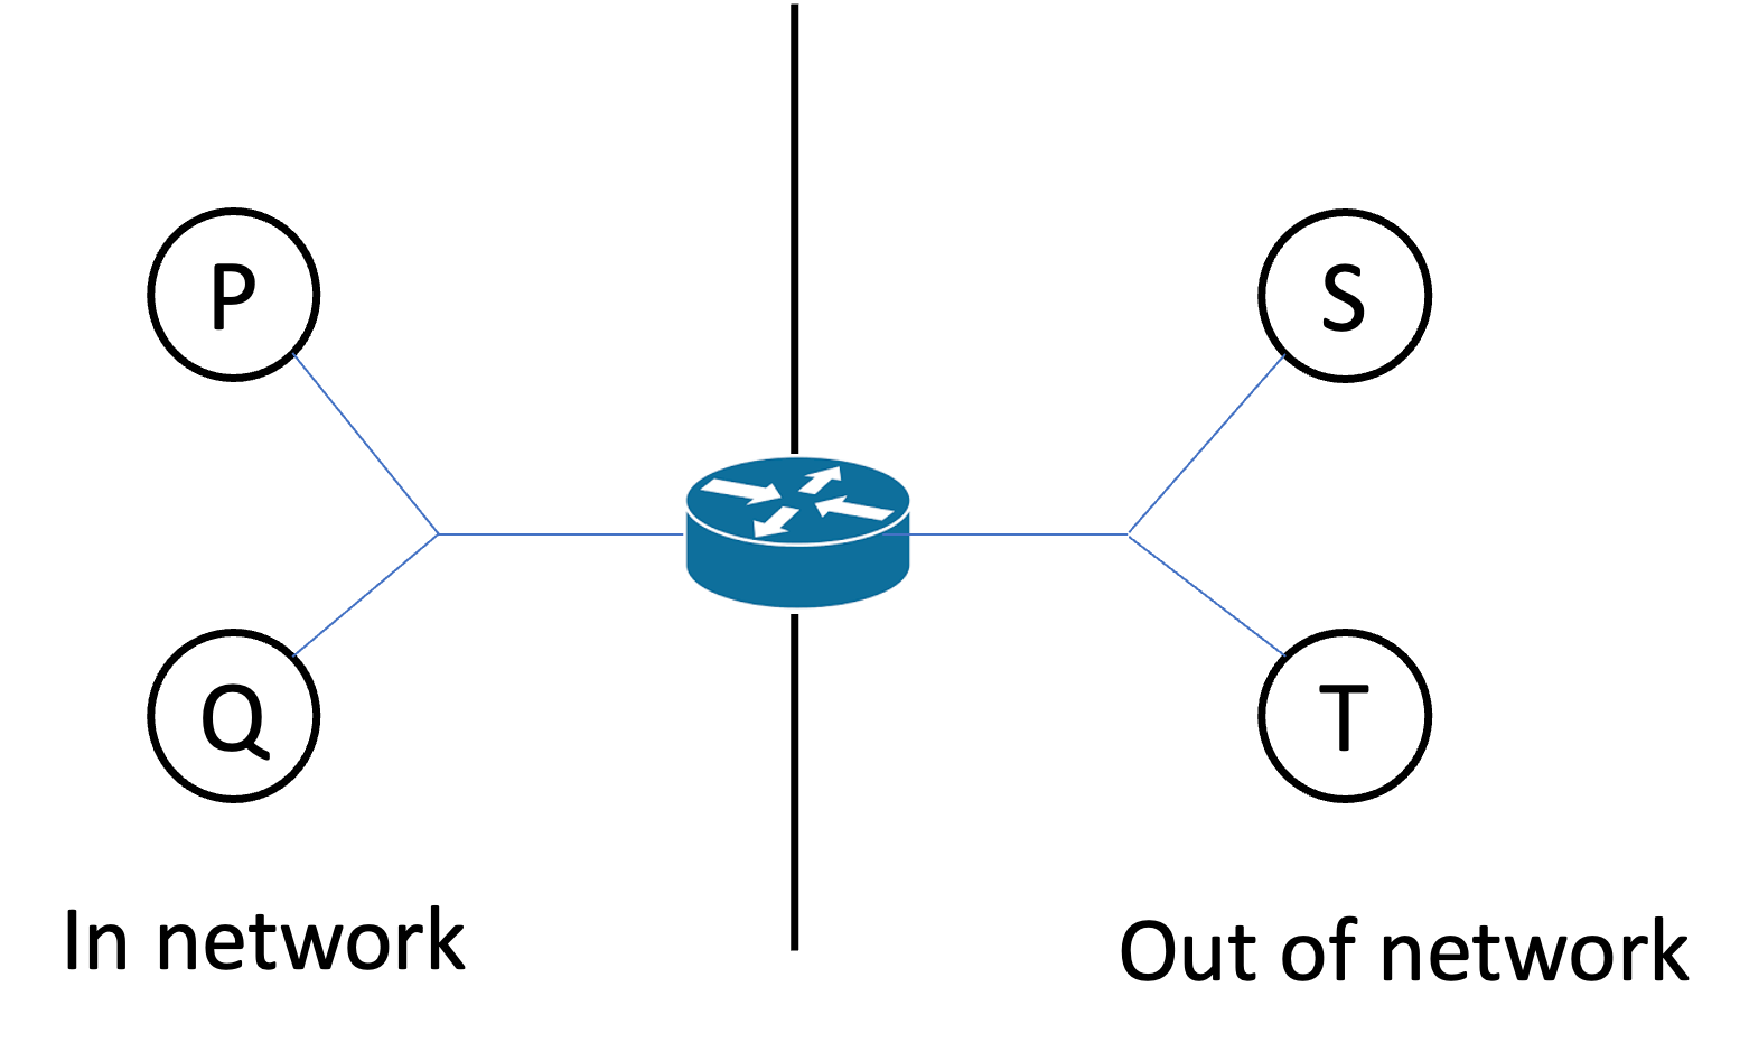
\includegraphics[scale=0.23]{figures/firewall.pdf}
    \label{fig:firewall}
\end{figure}
    
    Our firewall applies different rules based on the contents of the packet headers. The following table lists the criteria to identify the packet function.
    
    \hspace*{10mm} \textbf{mail}: Dst. port = 25
    
    \hspace*{10mm} \textbf{file transfer}: Dst. port = 20
    
    \hspace*{10mm} \textbf{TCP acknowledgements}: TCP\_ack flag is set
    
    \hspace*{10mm} \textbf{remote login request}: Dst. port = 22
    
    Fill in the table below based on the following rules. The rules are in order of least to greatest cost.
    
    \hspace*{10mm} Apply Rule \textbf{R1} when S sends mail to P
    
    \hspace*{10mm} Apply Rule \textbf{R2} when T transfers files to any device in the network
    
    \hspace*{10mm} Apply Rule \textbf{R3} when S sends a remote login request to any device in the network
    
    \hspace*{10mm} Apply Rule \textbf{R4} for any traffic originating from the network
    
    \hspace*{10mm} Apply Rule \textbf{R5} when any device sends a TCP acknowledgement to any device in the network
    
    \hspace*{10mm} Apply Rule \textbf{R6} for any traffic at all
    

\begin{table}[ht]
\begin{center}
\begin{tabular}{|c|p{1.8cm}|p{1.8cm}|c|c|c|}
	\hline
	Rule & Dst IP & Src IP & Dst Port & Src Port & Flags \\
	\hline
	R1 & D1 = 0101 & S1 = 1010 & 25 & - & - \\
	\hline
    R2 & D2 = 01* & S2 = 1101 & 20 & - & - \\
	\hline
    R3 & D3 = 01* & S3 = 1010 & 22 & - & - \\
	\hline
	R4 & D4 = * & S4 = 01* & * & - & - \\
	\hline
	R5 & D5 = 01* & S5 = * & * & - & TCP ack\\
	\hline
	R6 & D6 = * & S6 = * & * & * & * \\
	\hline
	
\end{tabular}
\end{center}
\end{table}
    
\item Similar to in class, let's solve a simpler problem by only focusing on classifying packets based on the source and destination IP addresses. In other words, take the table you filled in above, and for this sub-problem, only consider the columns for Rule, Dst IP, and Src IP.

Your task here is to draw two versions of the trie of tries. 
\begin{enumerate}
    \item The first version is the one you would use with the backtracking algorithm. Similar to class, we start with the destination trie at the top, and each valid prefix points to a source trie. In this version, each of \{S1, S2, ..., S6\} is present in exactly one source trie.
    \item In the second version, once the algorithm follows a pointer to a source trie, it does not leave that trie, so each trie must contain all necessary entries from \{S1, S2, ..., S6\}. Similar to class, we start with the destination trie at the top, and each valid prefix points to a source trie. 
\end{enumerate}
Notes: In both drawings, please distinguish clearly between destination and source tries, i.e., different color or dashed lines between them. Please also label which nodes in the source trie correspond to rules by labelling them, i.e., R1, R2, etc. If a node matches multiple rules, only label it with the best rule. Finally, remember to add arrows such that \textbf{every} destination trie node points to the source trie corresponding to its best matching prefix.
\end{enumerate}
\end{problem}

\subsection*{Answer 2:}


\begin{problem}{3: Reading}
We looked at firewalls in Problem 2, but another reason to look at multiple fields in a packet header is treat certain traffic differently with regards to quality of service. Your reading assignment this week is to research the problem of network neutrality. Then, write an explanation to a friend (2-3 paragraphs) who understands basic networking terms but does not know what net neutrality is, explaining the following 1) How does network discrimination work? 2) What are the main arguments for and against net neutrality?

I found \href{https://www.cs.princeton.edu/courses/archive/fall21/cos109/neutrality.pdf}{this} article to be helpful in presenting the technical details, but you may use any source you'd like (please cite the sources you used).
\end{problem}
\begin{problem}{4}
How long did this assignment take you?
\end{problem}
\end{document}

